\documentclass[xcolor={dvipsnames}]{beamer}

\usepackage{natbib}
\usepackage{amsmath}
\usepackage{amssymb}
\usepackage[scale=2]{ccicons}
\usepackage{appendixnumberbeamer}
\usepackage{booktabs}
\usepackage{graphicx}
\usepackage{hyperref}
\usepackage{extarrows}

% absolute positioning
\usepackage[absolute,overlay]{textpos}

%tikz stuff
\usepackage{tikz}
\usetikzlibrary{arrows}

% node styles
\tikzstyle{Endogenous}=[minimum size=0.7cm, fill=white, line width = 0.5mm, draw=black, shape=circle, text=black]
\tikzstyle{Policy}=[minimum size=0.7cm, fill=white, line width = 0.5mm, draw=blue, shape=circle, text=blue]
\tikzstyle{Confounder}=[minimum size=0.7cm, fill=white, line width = 0.5mm, draw=red, shape=circle, text=red]
\tikzstyle{Instrument}=[minimum size=0.7cm, fill=white, line width = 0.5mm, draw=Plum, shape=circle, text=Plum]

% Edge styles
\tikzstyle{arrow}=[line width = 0.5mm]


\pgfdeclarelayer{nodelayer}
\pgfdeclarelayer{edgelayer}
\pgfsetlayers{nodelayer, edgelayer}


\newcommand{\source}[1]{{\let\thefootnote\relax\footnote{{\tiny #1}}}}

% bf series
\def\bfA{\mathbf{A}}
\def\bfB{\mathbf{B}}
\def\bfC{\mathbf{C}}
\def\bfD{\mathbf{D}}
\def\bfE{\mathbf{E}}
\def\bfF{\mathbf{F}}
\def\bfG{\mathbf{G}}
\def\bfH{\mathbf{H}}
\def\bfI{\mathbf{I}}
\def\bfJ{\mathbf{J}}
\def\bfK{\mathbf{K}}
\def\bfL{\mathbf{L}}
\def\bfM{\mathbf{M}}
\def\bfN{\mathbf{N}}
\def\bfO{\mathbf{O}}
\def\bfP{\mathbf{P}}
\def\bfQ{\mathbf{Q}}
\def\bfR{\mathbf{R}}
\def\bfS{\mathbf{S}}
\def\bfT{\mathbf{T}}
\def\bfU{\mathbf{U}}
\def\bfV{\mathbf{V}}
\def\bfW{\mathbf{W}}
\def\bfX{\mathbf{X}}
\def\bfY{\mathbf{Y}}
\def\bfZ{\mathbf{Z}}

% bb series
\def\bbA{\mathbb{A}}
\def\bbB{\mathbb{B}}
\def\bbC{\mathbb{C}}
\def\bbD{\mathbb{D}}
\def\bbE{\mathbb{E}}
\def\bbF{\mathbb{F}}
\def\bbG{\mathbb{G}}
\def\bbH{\mathbb{H}}
\def\bbI{\mathbb{I}}
\def\bbJ{\mathbb{J}}
\def\bbK{\mathbb{K}}
\def\bbL{\mathbb{L}}
\def\bbM{\mathbb{M}}
\def\bbN{\mathbb{N}}
\def\bbO{\mathbb{O}}
\def\bbP{\mathbb{P}}
\def\bbQ{\mathbb{Q}}
\def\bbR{\mathbb{R}}
\def\bbS{\mathbb{S}}
\def\bbT{\mathbb{T}}
\def\bbU{\mathbb{U}}
\def\bbV{\mathbb{V}}
\def\bbW{\mathbb{W}}
\def\bbX{\mathbb{X}}
\def\bbY{\mathbb{Y}}
\def\bbZ{\mathbb{Z}}

% cal series
\def\calA{\mathcal{A}}
\def\calB{\mathcal{B}}
\def\calC{\mathcal{C}}
\def\calD{\mathcal{D}}
\def\calE{\mathcal{E}}
\def\calF{\mathcal{F}}
\def\calG{\mathcal{G}}
\def\calH{\mathcal{H}}
\def\calI{\mathcal{I}}
\def\calJ{\mathcal{J}}
\def\calK{\mathcal{K}}
\def\calL{\mathcal{L}}
\def\calM{\mathcal{M}}
\def\calN{\mathcal{N}}
\def\calO{\mathcal{O}}
\def\calP{\mathcal{P}}
\def\calQ{\mathcal{Q}}
\def\calR{\mathcal{R}}
\def\calS{\mathcal{S}}
\def\calT{\mathcal{T}}
\def\calU{\mathcal{U}}
\def\calV{\mathcal{V}}
\def\calW{\mathcal{W}}
\def\calX{\mathcal{X}}
\def\calY{\mathcal{Y}}
\def\calZ{\mathcal{Z}}

\newcommand{\argdot}{{\,\vcenter{\hbox{\tiny$\bullet$}}\,}} %generic argument dot

% easy bracketing:
\newcommand{\rbr}[1]{\left(#1\right)}
\newcommand{\sbr}[1]{\left[#1\right]}
\newcommand{\cbr}[1]{\left\{#1\right\}}
\newcommand{\abr}[1]{\left\langle#1\right\rangle}

% Norms
\def\norm#1{\|#1\|}
\def\biggnorm#1{\bigg\|#1\bigg\|}
% Random Variable Norms:
\def\psitwo#1{\|#1\|_{\psi_2}}
\def\psione#1{\|#1\|_{\psi_1}}

% mid
\newcommand{\biggmid}{\bigg \vert }

% argmax/argmin
\def\argmax{\mathop{\rm arg\,max}}
\def\argmin{\mathop{\rm arg\,min}}

% General Symbols
\def\half{\frac 1 2}
\newcommand{\halved}[1]{\frac{#1}{2}}
\newcommand{\R}{\mathbb{R}}

\newcommand{\into}{\rightarrow}

% Gradient Descent Symbols

% iterates
\newcommand{\w}{w}
\newcommand{\wk}{w_k}
\newcommand{\wkk}{w_{k+1}}
\newcommand{\wopt}{w^*}
% noise
\newcommand{\z}{Z}
\newcommand{\zk}{Z_k}
\newcommand{\zkk}{Z_{k+1}}
% step-sizes
\newcommand{\etak}{\eta_k}
\newcommand{\etakk}{\eta_{k+1}}

\newcommand{\E}{\bbE}

% functions
\newcommand{\f}{f}
\newcommand{\fj}{f_i}
\newcommand{\fopt}{f^*}
% sub-sampled functions
\newcommand{\fk}{f_{i_k}}
\newcommand{\fkk}{f_{i_{(k+1)}}}
% gradients
\newcommand{\grad}{\nabla f}
% sub-sampled gradients
\newcommand{\gradk}{\nabla f_{i_k}}
\newcommand{\gradkk}{\nabla f_{i_{(k+1)}}}


%%%%%%%%%%%%%%%%%%%%%%%%%%%%%%%%%%%%%%%%%%%%%%%%%%%%%%%%%%


\usepackage{simplebeam}

\newcommand{\policy}{\mbox{\textcolor{blue}{$P$}}}
\newcommand{\response}{\mbox{\textcolor{black}{$Y$}}}
\newcommand{\confounder}{\mbox{\textcolor{red}{$\epsilon$}}}
\newcommand{\features}{\mbox{\textcolor{black}{$X$}}}
\newcommand{\instrument}{\mbox{\textcolor{Plum}{$Z$}}}

\newcommand{\ind}{\perp\!\!\!\!\perp}

%Information to be included in the title page:
\title{Instrumental Variables, DeepIV, and Forbidden Regressions}

\author{Aaron Mishkin}
\institute{UBC MLRG 2019W2}
\date{}

\begin{document}

    \begin{frame}

        \titlepage

    \end{frame}

    \begin{frame}{Introduction}

            \begin{center}
                \Large \textbf{Goal}: Counterfactual reasoning in the presence of unknown confounders.
                \vspace{0.2cm}
                \begin{figure}
                    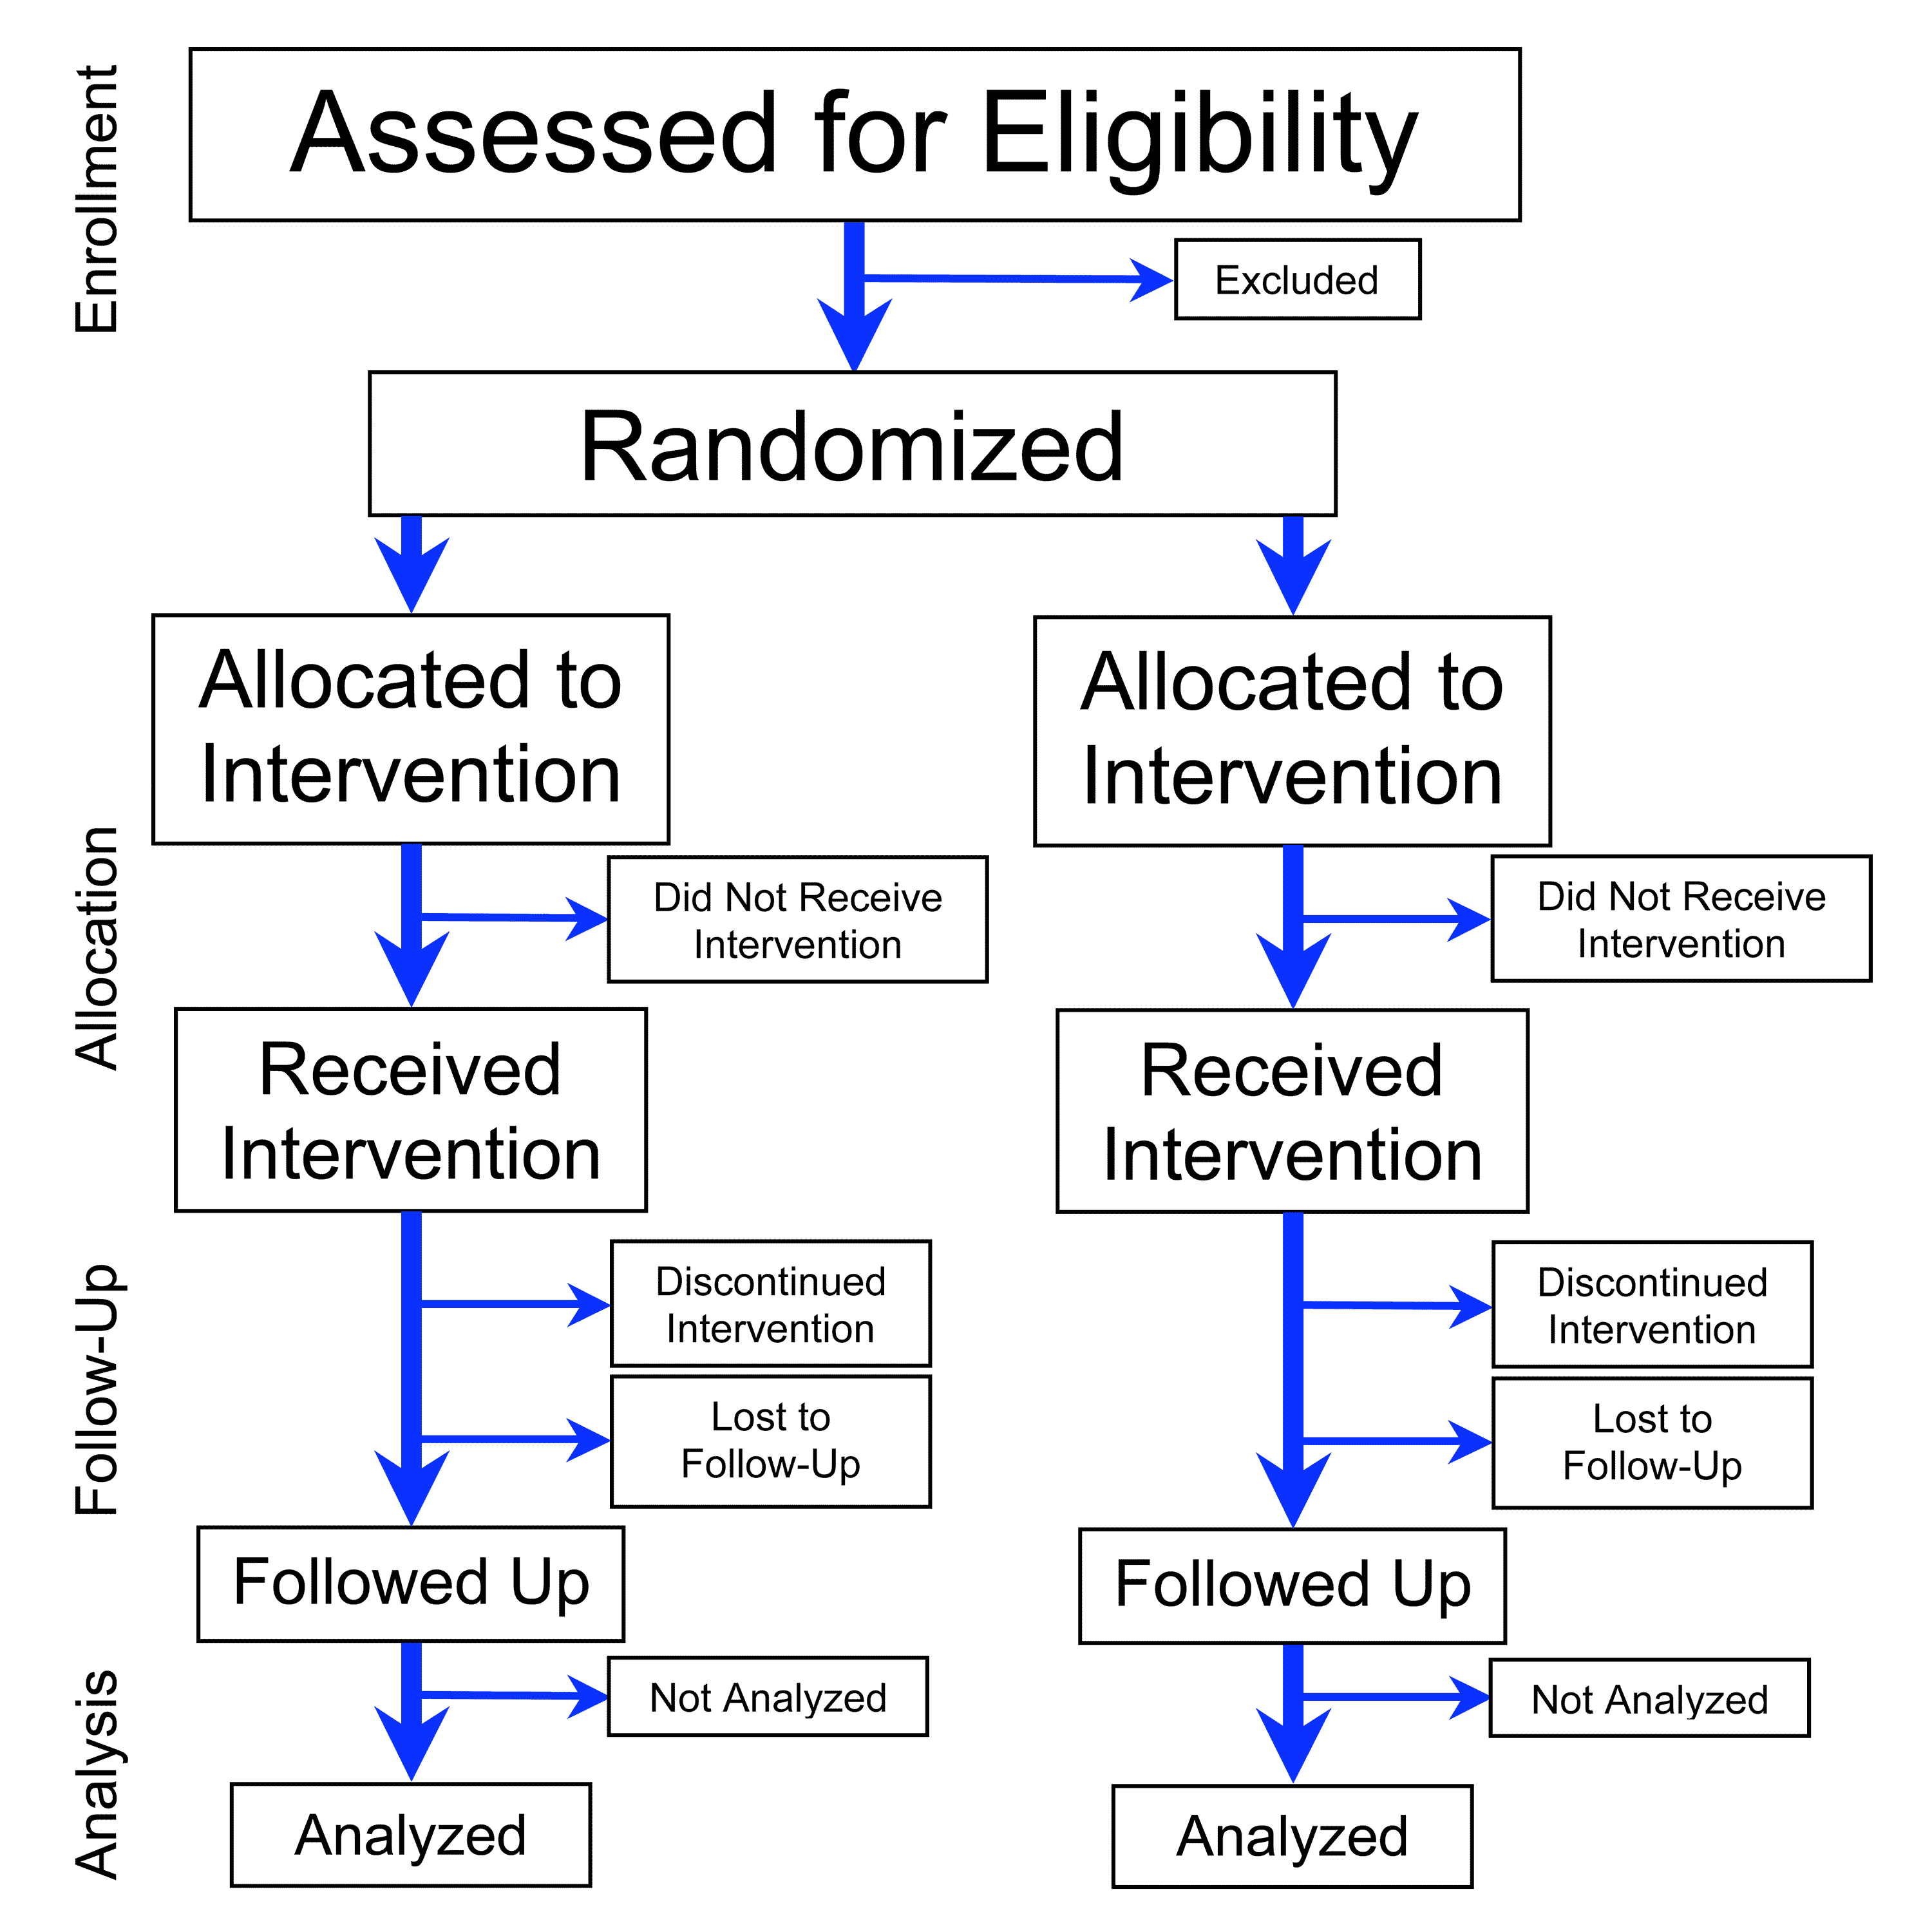
\includegraphics[width=0.5\textwidth]{figures/flow_chart}
                \end{figure}
            \end{center}

        \source{From the CONSORT 2010 statement~\citep{schulz2010consort}; https://commons.wikimedia.org/w/index.php?curid=9841081}

    \end{frame}

    \begin{frame}{Introduction: Motivation}

        \begin{center}
            \large Can we draw causal conclusions from observational data?
        \end{center}

        \vspace{0.3cm}

        \begin{itemize}
            \item \textbf{Medical Trials}: Is the new sunscreen I'm using effective?
            \begin{itemize}
                \item \textbf{Confounder}: I live in my laboratory!\vspace{0.2cm}
            \end{itemize}
            \item \textbf{Pricing}: should airlines increase ticket prices next December?
            \begin{itemize}
                \item \textbf{Confounder}: NeurIPS 2019 was in Vancouver.\vspace{0.2cm}
            \end{itemize}
            \item \textbf{Policy}: will unemployment continue to drop if the Federal Reserve keeps interest rates low?
            \begin{itemize}
                \item \textbf{Confounder}: US shale oil production increases.
            \end{itemize}
        \end{itemize}

        \vspace{0.3cm}

        \begin{center}
            \large We cannot control for confounders in observational data!
        \end{center}

    \end{frame}

    \begin{frame}{Introduction: Graphical Model}

        \begin{figure}
            \centering
            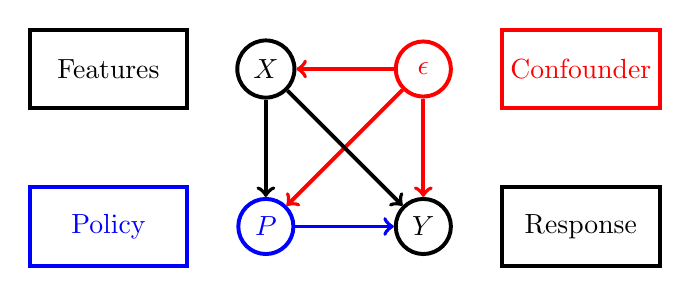
\begin{tikzpicture}
	\begin{pgfonlayer}{nodelayer}
		\node [style=Endogenous] (features) at (0, 2) {$X$};
		\node [style=Endogenous] (outcomes) at (2, 0) {$Y$};
		\node [style=Policy] (policy) at (0, 0) {$P$};
		\node [style=Confounder] (confounder) at (2, 2) {$\epsilon$};
	\end{pgfonlayer}
	\begin{pgfonlayer}{edgelayer}
		\draw [->, style=arrow, draw=red] (confounder) to (policy);
		\draw [->, style=arrow, draw=red] (confounder) to (outcomes);
		\draw [->, style=arrow, draw=red] (confounder) to (features);
		\draw [->, style=arrow, draw=blue] (policy) to (outcomes);
		\draw [->, style=arrow, draw=black] (features) to (outcomes);
		\draw [->, style=arrow, draw=black] (features) to (policy);

		% colored labels
		\draw [draw=red, line width = 0.5mm] (3,2.5) rectangle (5,1.5) node[pos=0.5] {\color{red}{Confounder}};
		\draw [draw=black, line width = 0.5mm] (3,0.5) rectangle (5,-0.5) node[pos=0.5] {\color{black}{Response}};
		\draw [draw=black, line width = 0.5mm] (-3,2.5) rectangle (-1,1.5) node[pos=0.5] {\color{black}{Features}};
		\draw [draw=blue, line width = 0.5mm] (-3,0.5) rectangle (-1,-0.5) node[pos=0.5] {\color{blue}{Policy}};
	\end{pgfonlayer}
\end{tikzpicture}

        \end{figure}

        We will graphical models to represent our learning problem.\vspace{0.2cm}
        \begin{itemize}
            \item \features{}: observed \emph{features} associated with a trial.
            \item \confounder{}: unobserved (possibly unknown) \emph{confounders}.
            \item \policy{}: the \emph{policy} variable we will to control.
            \item \response{}: the \emph{response} we want to predict.
        \end{itemize}

    \end{frame}

    \begin{frame}{Introduction: Answering Causal Questions}

        \begin{figure}
            \centering
            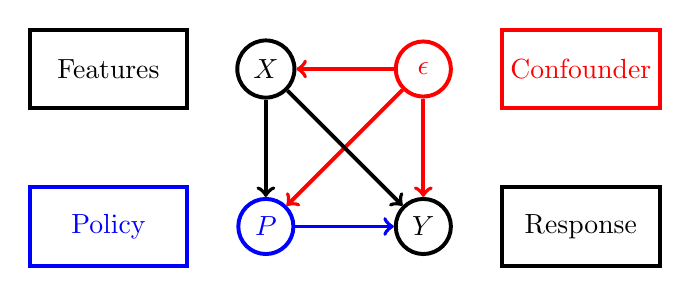
\begin{tikzpicture}
	\begin{pgfonlayer}{nodelayer}
		\node [style=Endogenous] (features) at (0, 2) {$X$};
		\node [style=Endogenous] (outcomes) at (2, 0) {$Y$};
		\node [style=Policy] (policy) at (0, 0) {$P$};
		\node [style=Confounder] (confounder) at (2, 2) {$\epsilon$};
	\end{pgfonlayer}
	\begin{pgfonlayer}{edgelayer}
		\draw [->, style=arrow, draw=red] (confounder) to (policy);
		\draw [->, style=arrow, draw=red] (confounder) to (outcomes);
		\draw [->, style=arrow, draw=red] (confounder) to (features);
		\draw [->, style=arrow, draw=blue] (policy) to (outcomes);
		\draw [->, style=arrow, draw=black] (features) to (outcomes);
		\draw [->, style=arrow, draw=black] (features) to (policy);

		% colored labels
		\draw [draw=red, line width = 0.5mm] (3,2.5) rectangle (5,1.5) node[pos=0.5] {\color{red}{Confounder}};
		\draw [draw=black, line width = 0.5mm] (3,0.5) rectangle (5,-0.5) node[pos=0.5] {\color{black}{Response}};
		\draw [draw=black, line width = 0.5mm] (-3,2.5) rectangle (-1,1.5) node[pos=0.5] {\color{black}{Features}};
		\draw [draw=blue, line width = 0.5mm] (-3,0.5) rectangle (-1,-0.5) node[pos=0.5] {\color{blue}{Policy}};
	\end{pgfonlayer}
\end{tikzpicture}

        \end{figure}

        \begin{itemize}
            \item \textbf{Causal Statements}: \response{} is caused by \policy{}.\vspace{0.2cm}
            \item \textbf{Action Sentences}: \response{} will happen if we \emph{do} \policy{}.\vspace{0.2cm}
            \item \textbf{Counterfactuals:} Given $(x, p, y)$ happened, how would \response{} change if we had \emph{done} \policy{} instead?\vspace{0.2cm}
        \end{itemize}

    \end{frame}

    \begin{frame}{Introduction: Berkeley Gender Bias Study}

        \textbf{S}: Gender causes admission to UC Berkeley~\citep{bickel1975sex}.\\
        \textbf{A}: Estimate mapping $g(\textcolor{blue}{p})$ from 1973 admissions records.

        \begin{figure}
            \centering
            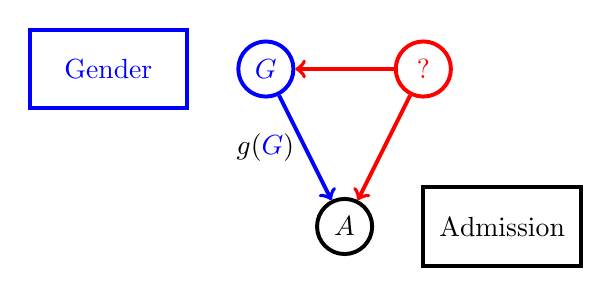
\begin{tikzpicture}
	\begin{pgfonlayer}{nodelayer}
		\node [style=Endogenous] (outcomes) at (1, 0) {$A$};
		\node [style=Policy] (policy) at (0, 2) {$G$};
		\node [style=Confounder] (confounder) at (2, 2) {?};
	\end{pgfonlayer}
	\begin{pgfonlayer}{edgelayer}
		\draw [->, style=arrow, draw=red] (confounder) to (policy);
		\draw [->, style=arrow, draw=red] (confounder) to (outcomes);
		\draw [->, style=arrow, draw=blue] (policy) to node[pos=0.5, left] {$g(\textcolor{blue}{G})$} (outcomes);

		% % colored labels
		% \draw [draw=red, line width = 0.5mm] (3,2.5) rectangle (5,1.5) node[pos=0.5] {\color{red}{Department}};
		\draw [draw=black, line width = 0.5mm] (2,0.5) rectangle (4,-0.5) node[pos=0.5] {\color{black}{Admission}};
		\draw [draw=blue, line width = 0.5mm] (-3,1.5) rectangle (-1,2.5) node[pos=0.5] {\color{blue}{Gender}};
	\end{pgfonlayer}
\end{tikzpicture}

        \end{figure}

        \begin{table}
            \centering
            \begin{tabular}{c c | c c}
                \multicolumn{2}{c |}{Men} & \multicolumn{2}{c}{Women} \\
                Applications & Admitted & Applications & Admitted \\ \hline
                8442 & 44\% & 4321 & 35\%
            \end{tabular}
        \end{table}

    \end{frame}

    \begin{frame}{Introduction: Berkeley with a Controlled Trial}
        \begin{figure}
            \centering
            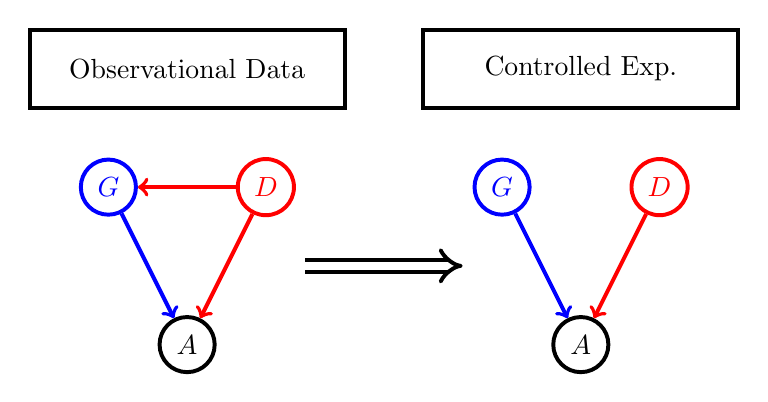
\begin{tikzpicture}
	\begin{pgfonlayer}{nodelayer}
		\node [style=Endogenous] (outcomes) at (1, 0) {$A$};
		\node [style=Policy] (policy) at (0, 2) {$G$};
		\node [style=Confounder] (confounder) at (2, 2) {$D$};
		% do model
		\node [style=Endogenous] (do_outcomes) at (6, 0) {$A$};
		\node [style=Policy] (do_policy) at (5, 2) {$G$};
		\node [style=Confounder] (do_confounder) at (7, 2) {$D$};
	\end{pgfonlayer}
	\begin{pgfonlayer}{edgelayer}
		\draw [->, style=arrow, draw=red] (confounder) to (policy);
		\draw [->, style=arrow, draw=red] (confounder) to (outcomes);
		\draw [->, style=arrow, draw=blue] (policy) to (outcomes);
		\draw [->, style=arrow, draw=red] (do_confounder) to (do_outcomes);
		\draw [->, style=arrow, draw=blue] (do_policy) to (do_outcomes);
		\draw [-implies, double distance=1mm, draw=black, line width=0.5mm] (2.5, 1) -- (4.5,1);

		% labels
		\draw [draw=black, line width = 0.5mm] (-1,4) rectangle (3,3) node[pos=0.5] {\color{black}{Observational Data}};
		\draw [draw=black, line width = 0.5mm] (4,4) rectangle (8,3) node[pos=0.5] {\color{black}{Controlled Exp.}};
	\end{pgfonlayer}
\end{tikzpicture}

        \end{figure}

        \begin{center}
            \textbf{Simpson's Paradox}: Controlling for the effects of \textcolor{red}{$D$} shows ``small but statistically significant bias in favor of women''~\citep{bickel1975sex}.
        \end{center}
    \end{frame}

    \setbeamercolor{background canvas}{bg=SkyBlue}
    \begin{frame}
        \begin{center}
            \Huge Part 1: ``Intervention Graphs''
        \end{center}
    \end{frame}
    \setbeamercolor{background canvas}{bg=white}

    \begin{frame}{Intervention Graphs}

        \begin{center}
            The $\text{do}(\cdot)$ operator formalizes this transformation~\citep{pearl2009causality}.
        \end{center}

        \begin{figure}
            \centering
            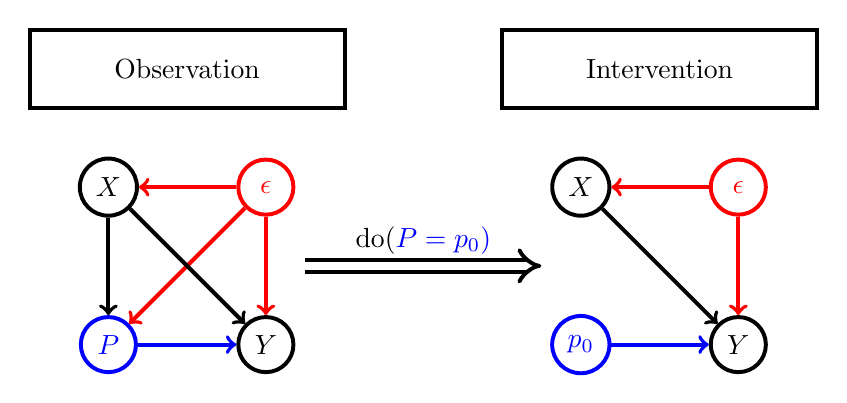
\begin{tikzpicture}
	\begin{pgfonlayer}{nodelayer}
		% basic model
		\node [style=Endogenous] (features) at (0, 2) {$X$};
		\node [style=Endogenous] (outcomes) at (2, 0) {$Y$};
		\node [style=Policy] (policy) at (0, 0) {$P$};
		\node [style=Confounder] (confounder) at (2, 2) {$\epsilon$};
		% do model
		\node [style=Endogenous] (do_features) at (6, 2) {$X$};
		\node [style=Endogenous] (do_outcomes) at (8, 0) {$Y$};
		\node [style=Policy] (do_policy) at (6, 0) {$p_0$};
		\node [style=Confounder] (do_confounder) at (8, 2) {$\epsilon$};
	\end{pgfonlayer}
	\begin{pgfonlayer}{edgelayer}
		% basic model
		\draw [->, style=arrow, draw=red] (confounder) to (policy);
		\draw [->, style=arrow, draw=red] (confounder) to (outcomes);
		\draw [->, style=arrow, draw=red] (confounder) to (features);
		\draw [->, style=arrow, draw=blue] (policy) to (outcomes);
		\draw [->, style=arrow, draw=black] (features) to (outcomes);
		\draw [->, style=arrow, draw=black] (features) to (policy);
		% do model
		\draw [->, style=arrow, draw=red] (do_confounder) to (do_outcomes);
		\draw [->, style=arrow, draw=red] (do_confounder) to (do_features);
		\draw [->, style=arrow, draw=blue] (do_policy) to (do_outcomes);
		\draw [->, style=arrow, draw=black] (do_features) to (do_outcomes);
		% joining operation
		\draw [-implies, double distance=1mm, draw=black, line width=0.5mm] (2.5, 1) -- node[above] {do$(\color{blue}{P = p_0})$} (5.5,1);

		% labels
		\draw [draw=black, line width = 0.5mm] (-1,4) rectangle (3,3) node[pos=0.5] {\color{black}{Observation}};
		\draw [draw=black, line width = 0.5mm] (5,4) rectangle (9,3) node[pos=0.5] {\color{black}{Intervention}};
	\end{pgfonlayer}
\end{tikzpicture}

        \end{figure}

        \textbf{Intuition}: effects of forcing \textcolor{blue}{$P = p_0$} vs ``natural'' occurrence.

    \end{frame}

    \begin{frame}{Intervention Graphs: Supervised vs Causal Learning}

        \begin{center} \Large \underline{Setup} \hspace{4cm} \underline{Graphical Model} \end{center}

        \begin{minipage}[c]{0.55\textwidth}
            \begin{itemize}
                \item \( \confounder{}, \textcolor{red}{\eta} \sim \calN\rbr{0,1} \).
                \item \( \policy{} = p + 2 \confounder{} \).
                \item \( g_0(\policy{}) = \max\cbr{\frac{\policy{}}{5}, \policy{}} \).
                \item \( \response{} = g_0(\policy{}) - 2 \confounder{} + \textcolor{red}{\eta} \).
            \end{itemize}
        \end{minipage}
        \begin{minipage}[c]{0.43\textwidth}
            \begin{figure}
                \centering
                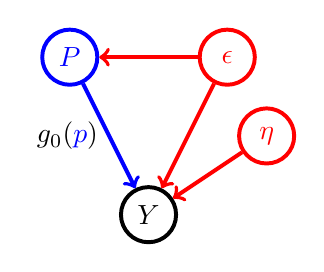
\begin{tikzpicture}
	\begin{pgfonlayer}{nodelayer}
		\node [style=Endogenous] (outcomes) at (1, 0) {$Y$};
		\node [style=Policy] (policy) at (0, 2) {$P$};
		\node [style=Confounder] (confounder) at (2, 2) {$\epsilon$};
		\node [style=Confounder] (noise) at (2.5, 1) {$\eta$};
	\end{pgfonlayer}
	\begin{pgfonlayer}{edgelayer}
		\draw [->, style=arrow, draw=red] (confounder) to (policy);
		\draw [->, style=arrow, draw=red] (noise) to (outcomes);
		\draw [->, style=arrow, draw=red] (confounder) to (outcomes);
		\draw [->, style=arrow, draw=blue] (policy) to node[pos=0.5, left] {$g_0(\textcolor{blue}{p})$} (outcomes);
	\end{pgfonlayer}
\end{tikzpicture}

            \end{figure}
        \end{minipage}

        \vspace{0.5cm}
        \begin{center}
            Can supervised learning recover \( g_0(\policy{} = \textcolor{blue}{p_0}) \) from observations?
        \end{center}

        \source{Synthetic example introduced by \citet{bennett2019deep}}

    \end{frame}

    \begin{frame}{Intervention Graphs: Supervised Failure}

        \begin{figure}
            \centering
            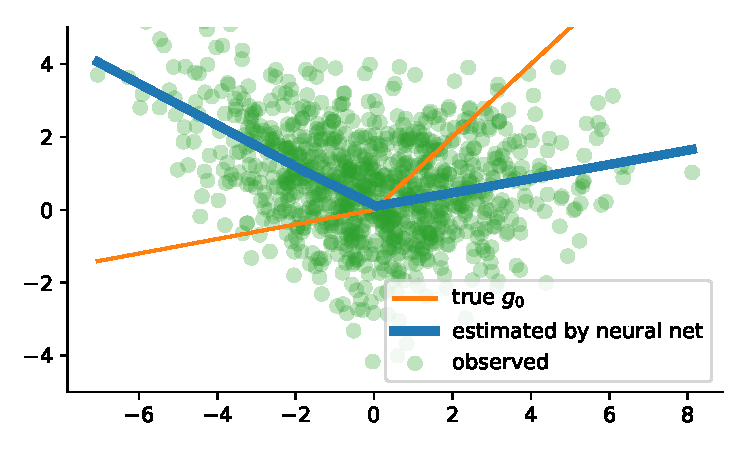
\includegraphics[width=0.8\textwidth]{figures/toy}
        \end{figure}

        \begin{center}
            \large Supervised learning fails because it assumes \( \policy{} \ind \confounder{} \)!
        \end{center}

        \source{Taken from https://arxiv.org/abs/1905.12495}

    \end{frame}

    \begin{frame}{Intervention Graphs: Supervised vs Causal Learning }

        \begin{figure}
            \centering
            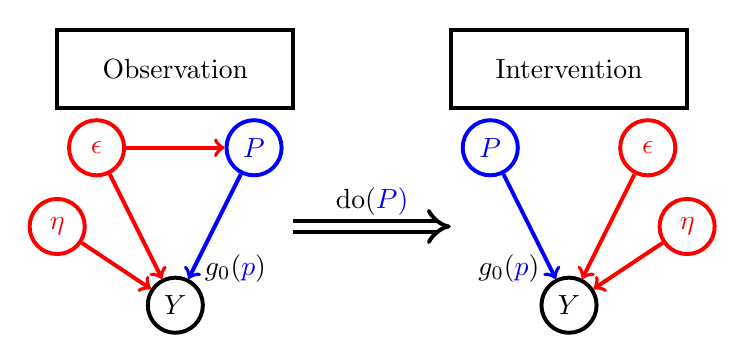
\begin{tikzpicture}
	\begin{pgfonlayer}{nodelayer}
		\node [style=Endogenous] (outcomes) at (1, 0) {$Y$};
		\node [style=Policy] (policy) at (2, 2) {$P$};
		\node [style=Confounder] (confounder) at (0, 2) {$\epsilon$};
		\node [style=Confounder] (noise) at (-0.5, 1) {$\eta$};
		% do model
		\node [style=Endogenous] (do_outcomes) at (6, 0) {$Y$};
		\node [style=Policy] (do_policy) at (5, 2) {$P$};
		\node [style=Confounder] (do_confounder) at (7, 2) {$\epsilon$};
		\node [style=Confounder] (do_noise) at (7.5, 1) {$\eta$};
	\end{pgfonlayer}
	\begin{pgfonlayer}{edgelayer}
		\draw [->, style=arrow, draw=red] (confounder) to (policy);
		\draw [->, style=arrow, draw=red] (noise) to (outcomes);
		\draw [->, style=arrow, draw=red] (confounder) to (outcomes);
		\draw [->, style=arrow, draw=blue] (policy) to node[pos=0.9, right] {$g_0(\textcolor{blue}{p})$} (outcomes);
		% do model
		\draw [->, style=arrow, draw=red] (do_noise) to (do_outcomes);
		\draw [->, style=arrow, draw=red] (do_confounder) to (do_outcomes);
		\draw [->, style=arrow, draw=blue] (do_policy) to node[pos=0.9, left] {$g_0(\textcolor{blue}{p})$} (do_outcomes);
		% implies
		\draw [-implies, double distance=1mm, draw=black, line width=0.5mm] (2.5, 1) -- node[above] {do$(\color{blue}{P})$} (4.5,1);
		% labels
		\draw [draw=black, line width = 0.5mm] (-0.5,3.5) rectangle (2.5,2.5) node[pos=0.5] {\color{black}{Observation}};
		\draw [draw=black, line width = 0.5mm] (4.5,3.5) rectangle (7.5,2.5) node[pos=0.5] {\color{black}{Intervention}};
	\end{pgfonlayer}
\end{tikzpicture}

        \end{figure}

        Given dataset \( \calD = \cbr{p_i, y_i}_{i=1}^n \):
        \begin{itemize}
            \item \textbf{Supervised Learning} estimates the conditional
            \[ \E \sbr{\response{} \mid \policy{}} = g_0(\policy{}) - 2 \E \sbr{\confounder{} \mid \policy{}} \]
            \item \textbf{Causal Learning} estimates the conditional
            \[ \E \sbr{\response{} \mid \text{do}{(\policy{})}} = g_0(\policy{}) -2 \underbrace{\E\sbr{\confounder{}}}_{=0}\]
        \end{itemize}
    \end{frame}


    \begin{frame}{Intervention Graphs: Known Confounders}

        \begin{figure}
            \centering
            
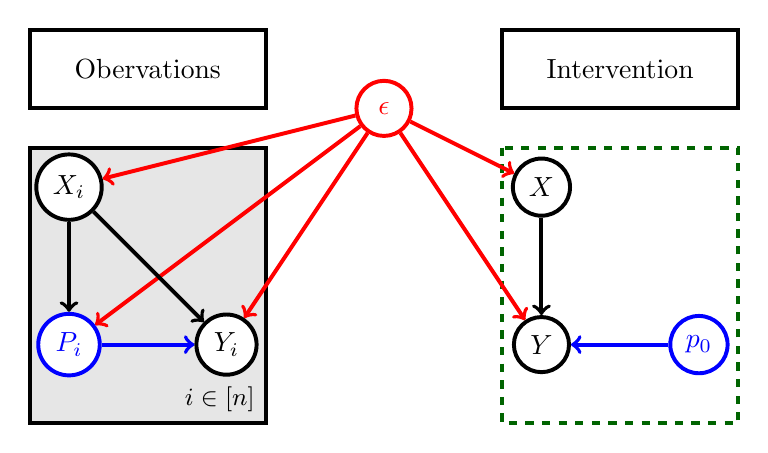
\begin{tikzpicture}
	\begin{pgfonlayer}{nodelayer}
		% plate
		\draw [line width = 0.5mm, fill=gray, fill opacity=0.2, text opacity=1](-1.5, 2.5) rectangle (1.5, -1) node[above left] {\small $i \in {[n]}$};

		\draw [line width = 0.5mm, draw=DarkGreen, dashed](4.5, 2.5) rectangle (7.5, -1);
		% basic model
		\node [style=Endogenous] (features) at (-1, 2) {$X_i$};
		\node [style=Endogenous] (outcomes) at (1, 0) {$Y_i$};
		\node [style=Policy] (policy) at (-1, 0) {$P_i$};
		\node [style=Confounder] (confounder) at (3, 3) {$\epsilon$};
		% do model
		\node [style=Endogenous] (do_features) at (5, 2) {$X$};
		\node [style=Endogenous] (do_outcomes) at (5, 0) {$Y$};
		\node [style=Policy] (do_policy) at (7, 0) {$p_0$};
	\end{pgfonlayer}
	\begin{pgfonlayer}{edgelayer}
		% basic model
		\draw [->, style=arrow, draw=red] (confounder) to (policy);
		\draw [->, style=arrow, draw=red] (confounder) to (outcomes);
		\draw [->, style=arrow, draw=red] (confounder) to (features);
		\draw [->, style=arrow, draw=blue] (policy) to (outcomes);
		\draw [->, style=arrow, draw=black] (features) to (outcomes);
		\draw [->, style=arrow, draw=black] (features) to (policy);
		% do model
		\draw [->, style=arrow, draw=red] (confounder) to (do_outcomes);
		\draw [->, style=arrow, draw=red] (confounder) to (do_features);
		\draw [->, style=arrow, draw=blue] (do_policy) to (do_outcomes);
		\draw [->, style=arrow, draw=black] (do_features) to (do_outcomes);

		% labels
		\draw [draw=black, line width = 0.5mm] (-1.5,4) rectangle (1.5,3) node[pos=0.5] {\color{black}{Obervations}};
		\draw [draw=black, line width = 0.5mm] (4.5,4) rectangle (7.5,3) node[pos=0.5] {\color{black}{Intervention}};
	\end{pgfonlayer}
\end{tikzpicture}

        \end{figure}

        What if
        \begin{enumerate}
            \item all confounders are known and in \confounder{};
            \item \confounder{} persists across observations;
            \item the mapping \( \response{} = f\,(\features{}, \policy{}, \confounder{})\) is known and persists.
        \end{enumerate}

    \end{frame}

    \begin{frame}{Intervention Graphs: Inference}

        \begin{figure}
            \centering
            
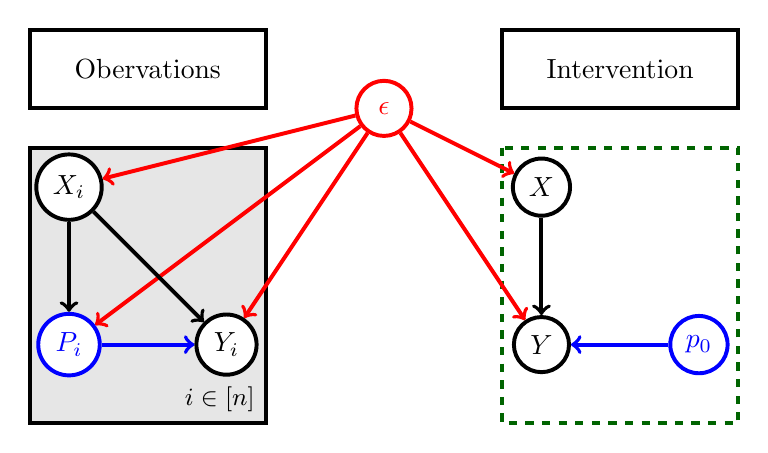
\begin{tikzpicture}
	\begin{pgfonlayer}{nodelayer}
		% plate
		\draw [line width = 0.5mm, fill=gray, fill opacity=0.2, text opacity=1](-1.5, 2.5) rectangle (1.5, -1) node[above left] {\small $i \in {[n]}$};

		\draw [line width = 0.5mm, draw=DarkGreen, dashed](4.5, 2.5) rectangle (7.5, -1);
		% basic model
		\node [style=Endogenous] (features) at (-1, 2) {$X_i$};
		\node [style=Endogenous] (outcomes) at (1, 0) {$Y_i$};
		\node [style=Policy] (policy) at (-1, 0) {$P_i$};
		\node [style=Confounder] (confounder) at (3, 3) {$\epsilon$};
		% do model
		\node [style=Endogenous] (do_features) at (5, 2) {$X$};
		\node [style=Endogenous] (do_outcomes) at (5, 0) {$Y$};
		\node [style=Policy] (do_policy) at (7, 0) {$p_0$};
	\end{pgfonlayer}
	\begin{pgfonlayer}{edgelayer}
		% basic model
		\draw [->, style=arrow, draw=red] (confounder) to (policy);
		\draw [->, style=arrow, draw=red] (confounder) to (outcomes);
		\draw [->, style=arrow, draw=red] (confounder) to (features);
		\draw [->, style=arrow, draw=blue] (policy) to (outcomes);
		\draw [->, style=arrow, draw=black] (features) to (outcomes);
		\draw [->, style=arrow, draw=black] (features) to (policy);
		% do model
		\draw [->, style=arrow, draw=red] (confounder) to (do_outcomes);
		\draw [->, style=arrow, draw=red] (confounder) to (do_features);
		\draw [->, style=arrow, draw=blue] (do_policy) to (do_outcomes);
		\draw [->, style=arrow, draw=black] (do_features) to (do_outcomes);

		% labels
		\draw [draw=black, line width = 0.5mm] (-1.5,4) rectangle (1.5,3) node[pos=0.5] {\color{black}{Obervations}};
		\draw [draw=black, line width = 0.5mm] (4.5,4) rectangle (7.5,3) node[pos=0.5] {\color{black}{Intervention}};
	\end{pgfonlayer}
\end{tikzpicture}

        \end{figure}

        Steps to inference:
        \begin{enumerate}
            \item \textbf{Abduction}: compute posterior \( P(\confounder{} \mid \cbr{x_i, \textcolor{blue}{p_i}, y_i}_{i=1}^n) \)
            \item \textbf{Action}: form subgraph corresponding to \( \text{do}(\policy{} = \textcolor{blue}{p_0}) \).
            \item \textbf{Prediction}: compute \( P(Y \mid \text{do}(\policy{} = \textcolor{blue}{p_0}), \cbr{x_i, p_i, y_i}_{i=1}^n) \).
        \end{enumerate}

    \end{frame}

    \begin{frame}{Intervention Graphs: Limitations}

        {\large Our assumptions are unrealistic since }
        \begin{itemize}
            \item identifying all confounders is \textbf{hard}.
            \item assuming all confounders are ``global'' is \textbf{unrealistic}.
            \item characterizing \( \response{} = f\,(\features{}, \policy{}, \confounder{}) \) requires \textbf{expert knowledge}.
        \end{itemize}

        \vspace{0.5cm}
        \large{ What we really want is to }
        \begin{itemize}
            \item allow \textbf{any} number and kind of confounders!
            \item allow confounders to be ``\textbf{local}''.
            \item \textbf{learn} \(f \,(\features{}, \policy{}, \confounder{}) \) from data!
        \end{itemize}
    \end{frame}

    \setbeamercolor{background canvas}{bg=SkyBlue}
    \begin{frame}
        \begin{center}
            \Huge Part 2: Instrumental Variables
        \end{center}
    \end{frame}
    \setbeamercolor{background canvas}{bg=white}

    \begin{frame}{Instrumental Variables}

        \begin{center}
            \Large \ldots the drawing of inferences from studies in which subjects have the final choice of program; the randomization is confined to an indirect \emph{instrument} (or assignment) that merely encourages or discourages participation in the various programs. \\
            ---~\citet{pearl2009causality}
        \end{center}

    \end{frame}

    \begin{frame}{IV: Expanded Model}

        \begin{figure}
            \centering
            
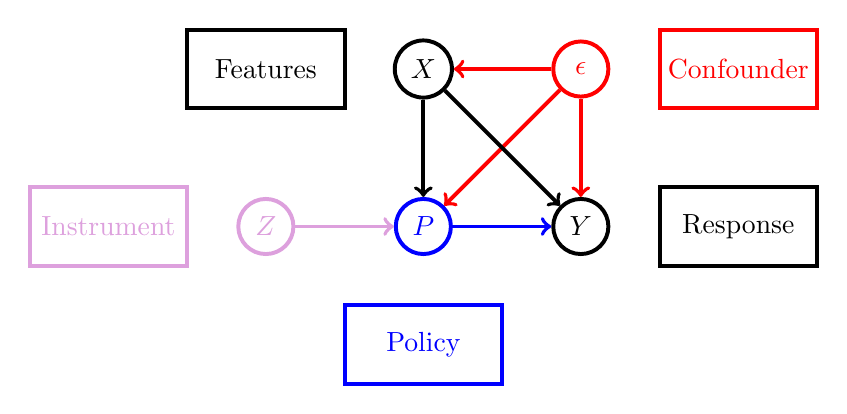
\begin{tikzpicture}
	\begin{pgfonlayer}{nodelayer}
		\node [style=Instrument] (instrument) at (-2, 0) {$Z$};
		\node [style=Endogenous] (features) at (0, 2) {$X$};
		\node [style=Endogenous] (outcomes) at (2, 0) {$Y$};
		\node [style=Policy] (policy) at (0, 0) {$P$};
		\node [style=Confounder] (confounder) at (2, 2) {$\epsilon$};
	\end{pgfonlayer}
	\begin{pgfonlayer}{edgelayer}
		\draw [->, style=arrow, draw=red] (confounder) to (policy);
		\draw [->, style=arrow, draw=red] (confounder) to (outcomes);
		\draw [->, style=arrow, draw=red] (confounder) to (features);
		\draw [->, style=arrow, draw=blue] (policy) to (outcomes);
		\draw [->, style=arrow, draw=black] (features) to (outcomes);
		\draw [->, style=arrow, draw=black] (features) to (policy);
		\draw [->, style=arrow, draw=Plum] (instrument) to (policy);

		% colored labels
		\draw [draw=red, line width = 0.5mm] (3,2.5) rectangle (5,1.5) node[pos=0.5] {\color{red}{Confounder}};
		\draw [draw=black, line width = 0.5mm] (3,0.5) rectangle (5,-0.5) node[pos=0.5] {\color{black}{Response}};
		\draw [draw=black, line width = 0.5mm] (-3,2.5) rectangle (-1,1.5) node[pos=0.5] {\color{black}{Features}};
		\draw [draw=blue, line width = 0.5mm] (-1,-1) rectangle (1,-2) node[pos=0.5] {\color{blue}{Policy}};
		\draw [draw=Plum, line width = 0.5mm] (-5,0.5) rectangle (-3,-0.5) node[pos=0.5] {\color{Plum}{Instrument}};
	\end{pgfonlayer}
\end{tikzpicture}

        \end{figure}

        We augment our model with an \emph{instrumental variable} \instrument{} that
        \begin{itemize}
            \item affects the distribution of \policy{};
            \item only affects \response{} through \policy{};
            \item is conditionally independent of \confounder{}.
        \end{itemize}

    \end{frame}

    \begin{frame}{IV: Air Travel Example}

        \begin{figure}
            \centering
            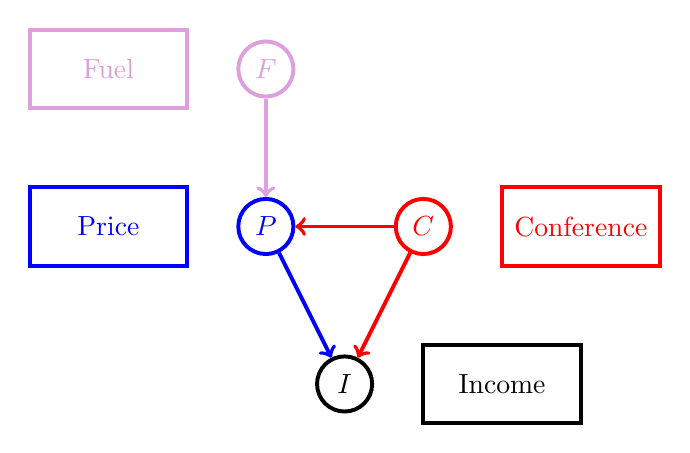
\begin{tikzpicture}
	\begin{pgfonlayer}{nodelayer}
		\node [style=Endogenous] (outcomes) at (1, 0) {$I$};
		\node [style=Policy] (policy) at (0, 2) {$P$};
		\node [style=Confounder] (confounder) at (2, 2) {$C$};
		\node [style=Instrument] (instrument) at (0, 4) {$F$};
	\end{pgfonlayer}
	\begin{pgfonlayer}{edgelayer}
		\draw [->, style=arrow, draw=red] (confounder) to (policy);
		\draw [->, style=arrow, draw=red] (confounder) to (outcomes);
		\draw [->, style=arrow, draw=blue] (policy) to (outcomes);
		\draw [->, style=arrow, draw=Plum] (instrument) to (policy);

		% colored labels
		\draw [draw=red, line width = 0.5mm] (3,2.5) rectangle (5,1.5) node[pos=0.5] {\color{red}{Conference}};
		\draw [draw=black, line width = 0.5mm] (2,0.5) rectangle (4,-0.5) node[pos=0.5] {\color{black}{Income}};
		\draw [draw=blue, line width = 0.5mm] (-3,1.5) rectangle (-1,2.5) node[pos=0.5] {\color{blue}{Price}};
		\draw [draw=Plum, line width = 0.5mm] (-3,3.5) rectangle (-1,4.5) node[pos=0.5] {\color{Plum}{Fuel}};
	\end{pgfonlayer}
\end{tikzpicture}

        \end{figure}

        \textbf{Intuition}: ``[\textcolor{Plum}{$F$} is] as good as randomization for the purposes of causal inference''---~\citet{hartford2017deep}.

    \end{frame}

    \begin{frame}{IV: Formally}
        \textbf{Goal}: counterfactual predictions of the form
        \[ \E \sbr{Y \mid \features{}, \, \text{do}(\policy{} = \textcolor{blue}{p_0})} - \E \sbr{Y \mid \features{}, \, \text{do}(\policy{} = \textcolor{blue}{p_1})}. \vspace{0.5cm}\]

        Let's make the following assumptions:
        \begin{enumerate}
            \item the additive noise model \( \response{} = g\, (\policy, \features) + \confounder{} \),\vspace{0.3cm}
            \item the following conditions on the IV:\vspace{0.2cm}
            \begin{enumerate}
                \item \textbf{Relevance}: \( p(\policy{} \mid \features{}, \instrument{}) \) is not constant in \instrument{}.\vspace{0.2cm}
                \item \textbf{Exclusion}: \( \instrument{} \ind \response{} \mid \policy{}, \features{}, \confounder{} \).\vspace{0.2cm}
                \item \textbf{Unconfounded Instrument}: \( \instrument{} \ind \confounder{} \mid \policy{} \).
            \end{enumerate}
        \end{enumerate}

    \end{frame}

    \begin{frame}{IV: Model Learning Part 1}

        \begin{figure}
            \centering
            
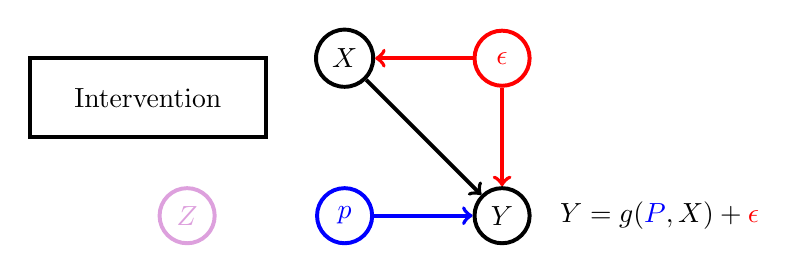
\begin{tikzpicture}
	\begin{pgfonlayer}{nodelayer}
		\node [style=Instrument] (instrument) at (-2, 0) {$Z$};
		\node [style=Endogenous] (features) at (0, 2) {$X$};
		\node [style=Endogenous] (outcomes) at (2, 0) {$Y$};
		\node [style=Policy] (policy) at (0, 0) {$p$};
		\node [style=Confounder] (confounder) at (2, 2) {$\epsilon$};
		\node [] (mapping) at (4,0) {$Y = g(\policy{}, \features{}) + \confounder{}$};
	\end{pgfonlayer}
	\begin{pgfonlayer}{edgelayer}
		\draw [->, style=arrow, draw=red] (confounder) to (outcomes);
		\draw [->, style=arrow, draw=red] (confounder) to (features);
		\draw [->, style=arrow, draw=blue] (policy) to (outcomes);
		\draw [->, style=arrow, draw=black] (features) to (outcomes);

		\draw [draw=black, line width = 0.5mm] (-4, 1) rectangle (-1, 2) node[pos=0.5] {Intervention};
	\end{pgfonlayer}
\end{tikzpicture}

        \end{figure}

        Under the do operator:
        \begin{align*}
            \E \sbr{Y \mid \features{}, \, \text{do}(\policy{} = \textcolor{blue}{p_0})} - \E \sbr{Y \mid \features{}, \, \text{do}(\policy{} = \textcolor{blue}{p_1})} &= g(\textcolor{blue}{p_0}, X) - g(\textcolor{blue}{p_1}, X)\\
            &  \quad+ \underbrace{\E\sbr{\confounder{} - \confounder{} \mid X}}_{=0}.
        \end{align*}

        So, we only need to estimate \( h(\policy{}, \features{}) = g(\textcolor{blue}{\policy{}}, X) + \E\sbr{\confounder{} \mid X}\)!

    \end{frame}

    \begin{frame}{IV: Model Learning Part 2}
        \textbf{Want}: \( h(\policy{}, \features{}) = g(\textcolor{blue}{\policy{}}, X) + \E\sbr{\confounder{} \mid X}\).

        \vspace{0.25cm}

        \textbf{Approach}: Marginalize out confounded policy \policy{}.\vspace{0.1cm}
        \begin{align*}
            \E \sbr{\response{} \mid \features{}, \instrument{} \, } &= \int_{\policy{}} \rbr{g\,(\textcolor{blue}{\policy{}}, X) + \E\sbr{\confounder{} \mid \policy{}, X}} d p(\policy{} \mid \features{}, \instrument{} \,)\\
            &= \int_{\policy{}} \rbr{g\,(\textcolor{blue}{\policy{}}, X) + \E\sbr{\confounder{} \mid X}} d p(\policy{} \mid \features{}, \instrument{} \,)\\
            &= \int_{\policy{}} h(\policy{}, \features{}) d p(\policy{} \mid \features{}, \instrument{} \,).\vspace{0.25cm}
        \end{align*}
        \textbf{Key Trick}: \( \E\sbr{\confounder{} \mid X} \) is the same as \( \E\sbr{\confounder{} \mid \policy{}, X} \) when marginalizing.\vspace{0.5cm}
    \end{frame}

    \begin{frame}{IV: Two-Stage Methods}
        \[\textbf{Objective}: \quad \frac{1}{n} \sum_{i=1}^n \calL\rbr{y_i, \int_{\policy{}} h(\policy{}, x_i) d p(\policy{} \mid \textcolor{Plum}{z_i} \,)}. \]

        \vspace{0.5cm}Two-stage methods:
        \begin{enumerate}
            \item \textbf{Estimate Density}: learn \( \hat p\,(\policy{} \mid \features{}, \instrument{}\,) \) from \(D = \cbr{\textcolor{blue}{p_i}, x_i, \textcolor{Plum}{z_i}}_{i=1}^n \).\vspace{0.2cm}
            \item \textbf{Estimate Function}: learn \( \hat h(\policy{}, \features{}) \) from \(\bar D = \cbr{y_i, x_i, \textcolor{Plum}{z_i}}_{i=1}^n \).\vspace{0.2cm}
            \item \textbf{Evaluate}: counterfactual reasoning via \( \hat h\,(\textcolor{blue}{p_0}, x) - \hat h\,(\textcolor{blue}{p_1}, x) \).\vspace{0.2cm}
        \end{enumerate}

    \end{frame}

    \begin{frame}{IV: Two-Stage Least-Squares}
        \textbf{Classic Approach}: two-stage least-squares (2SLS).\vspace{0.2cm}
        \begin{align*}
            h(\policy{}, \features{}) &= \mathbf{w}_0^\top \policy{} + \mathbf{w}_1^\top \features{} + \confounder{}\\
            \E[\policy{} \mid \features{}, \instrument{}] &= \mathbf{A}_0 \features{} + \mathbf{A}_1 \instrument{} + r\,(\confounder{})
        \end{align*}\vspace{0.2cm}
        Then we have the following:
        \vspace{-0.2cm}
        \begin{align*}
            \E \sbr{\response{} \mid \features{}, \instrument{} \, } &= \int_{\policy{}} h(\policy{}, \features{}) d p(\policy{} \mid \features{}, \instrument{} \,)\\
            &= \int_{\policy{}} \rbr{\mathbf{w}_0^\top \policy{} + \mathbf{w}_1^\top \features{}} d p(\policy{} \mid \features{}, \instrument{} \,)\\
            &= \mathbf{w}_1^\top \features{} + \mathbf{w}_0^\top \int_{\policy{}} \policy{} d p(\policy{} \mid \features{}, \instrument{} \,)\\
            &= \mathbf{w}_1^\top \features{} + \mathbf{w}_0^\top \rbr{\mathbf{A}_0 \features{} + \mathbf{A}_1 \instrument{}}.
        \end{align*}

        No need for density estimation!

        \source{See~\citet{angrist2008mostly}.}

    \end{frame}

    \setbeamercolor{background canvas}{bg=SkyBlue}
    \begin{frame}
        \begin{center}
            \Huge Part 3: Deep IV
        \end{center}
    \end{frame}
    \setbeamercolor{background canvas}{bg=white}

    \begin{frame}{Deep IV: Problems with 2SLS}
        \textbf{Problem}: Linear models aren't very expressive.
        \begin{itemize}
            \item What if we want to do causal inference with time-series?
        \end{itemize}

        \begin{figure}
            \centering
            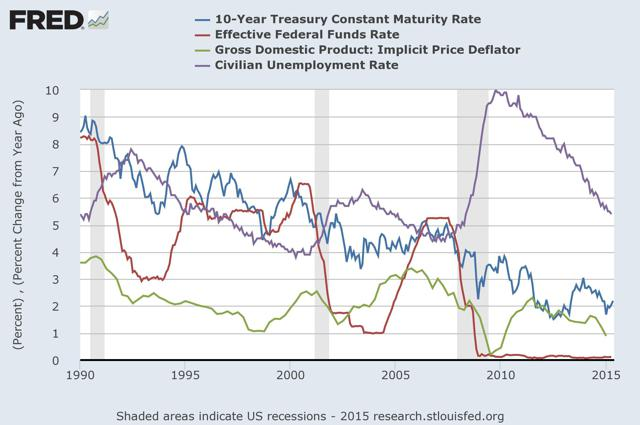
\includegraphics[width=0.88\textwidth]{figures/interest_vs_unemployment}
        \end{figure}

        \source{Federal Reserve Economic Research, Federal Reserve Bank of Saint Louis. https://fred.stlouisfed.org/}

    \end{frame}

    \begin{frame}{Deep IV: Problems with 2SLS}
        \textbf{Problem}: Linear models aren't very expressive.
        \begin{itemize}
            \item How about complex image data?
        \end{itemize}

        \begin{figure}
            \centering
            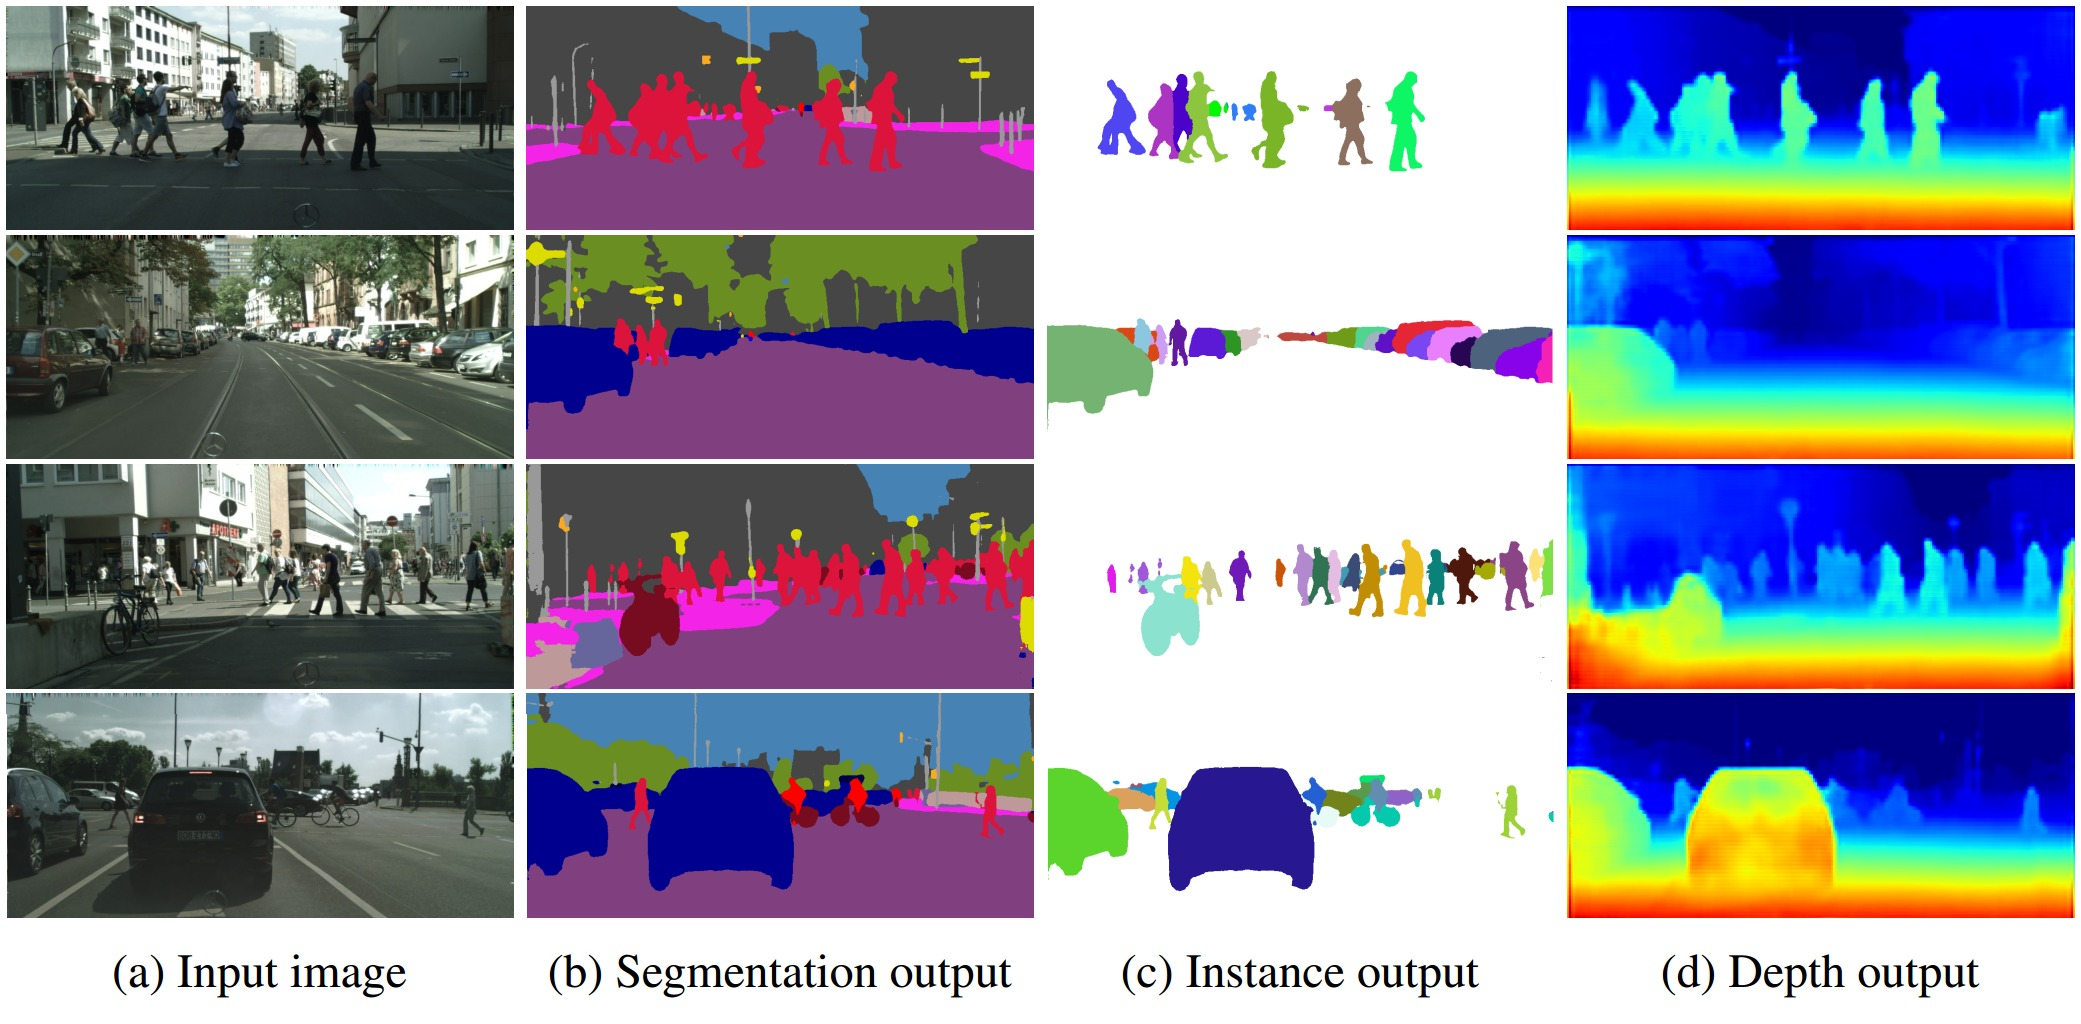
\includegraphics[width=0.95\textwidth]{figures/scene_understanding}
        \end{figure}

        \source{https://alexgkendall.com/computer\_vision/bayesian\_deep\_learning\_for\_safe\_ai/}

    \end{frame}

    \begin{frame}{Deep IV: Approach}
        Remember our objective function:
        \[\textbf{Objective}: \quad \frac{1}{n} \sum_{i=1}^n \calL\rbr{y_i, \int_{\policy{}} h(\policy{}, x_i) d p(\policy{} \mid \textcolor{Plum}{z_i} \,)}. \]

        \vspace{0.25cm}\textbf{Deep IV}: Two-stage method using deep neural networks.

        \begin{enumerate}
            \item \textbf{Treatment Network}: estimate \( \hat p \,(\policy{} \mid \phi(\features{}, \instrument{})\,) \).\vspace{0.2cm}
            \begin{itemize}
                \item \textbf{Categorical} \policy{}: softmax w/ favourite architecture. \vspace{0.2cm}
                \item \textbf{Continuous} \policy{}: autoregressive models (MADE, RNADE, etc.), normalizing flows (MAF, IAF, etc) and so on.\vspace{0.2cm}
            \end{itemize}
            \item \textbf{Outcome Network}: fit favorite architecture
            \[ \hat h_\theta (\policy{}, \features{}) \approx h(\policy{}, \features{}). \]
        \end{enumerate}

        \source{Autogressive models: \citep{germain2015made,uria2013rnade}, Normalizing Flows: \citep{rezende2015variational, papamakarios2017masked, kingma2016improved}}

    \end{frame}

    \begin{frame}{Deep IV: Training Deep IV Models}

        \textbf{1. Treatment Network} ``easy'' via maximum-likelihood:
        \begin{align*}
            \phi^* = \argmax_{\phi} \cbr{ \sum_{i=1}^n \log \hat p \,(\textcolor{blue}{p_i} \mid \phi(x_i, \textcolor{Plum}{z_i})\,) }
        \end{align*}

        \textbf{2. Outcome Network}: Monte Carlo approximation for loss:
        \begin{align*}
            L(\theta) &= \frac{1}{n} \sum_{i=1}^n \calL\rbr{y_i, \int_{\policy{}} \hat h_\theta \,(\policy{}, \features{}) d \hat p \,(\policy{} \mid \phi(x_i, \textcolor{Plum}{z_i})\,)}\\
            &\approx \frac{1}{n} \sum_{i=1}^n \calL\rbr{y_i, \frac{1}{M} \sum_{j=1}^m \hat h_\theta \,(\textcolor{blue}{p_j}, x_i)} :=  {\hat L}(\theta),
        \end{align*}
        where \( \textcolor{blue}{p_j} \sim \hat p \,(\policy{} \mid \phi(x_i, \textcolor{Plum}{z_i})\,) \).

    \end{frame}

    \begin{frame}{Deep IV: Biased and Unbiased Gradients}
        When \( \calL(y, \hat y) = {(y - \hat y)}^2 \):
        \[ L(\theta) = \frac{1}{n} \sum_{i=1}^n \rbr{y_i - \int_{\policy{}} h(\policy{}, x_i) d p(\policy{} \mid \textcolor{Plum}{z_i} \,)}^2. \]
        If we use a single set of samples to estimate \( \E_{\hat p} \sbr{\hat h_\theta \,(\policy{}, x_i)} \):
        \begin{align*}
            \nabla \hat L(\theta)&\approx -2 \frac{1}{n} \sum_{i=1}^n \E_{\hat p} \sbr{y_i - \hat h_\theta \,(\policy{}, x_i) \nabla_\theta \hat h_\theta \,(\policy{}, x_i)}\\
            &\geq -2 \frac{1}{n} \sum_{i=1}^n \E_{\hat p} \sbr{y_i - \hat h_\theta \,(\policy{}, x_i)}  \E_{\hat p} \sbr{\nabla_\theta \hat h_\theta \,(\policy{}, x_i)} = \nabla_\theta L(\theta),
        \end{align*}
        by Jensen's inequality.

    \end{frame}

    \setbeamercolor{background canvas}{bg=SkyBlue}
    \begin{frame}
        \begin{center}
            \Huge Part 4: Experimental Results and Forbidden Techniques
        \end{center}
    \end{frame}
    \setbeamercolor{background canvas}{bg=white}

    \begin{frame}{Results: Price Sensitivity}

        \textbf{Synthetic Price Sensitivity}: \( \textcolor{DarkGreen}{\rho} \in [0,1] \) tunes confounding.
        \begin{itemize}
            \item \( \text{Customer Type: } S \in \cbr{1, \dots, 7}; \text{ Price Sensitivity: } \psi_t \)
            \item \( \instrument{} \sim \calN(0,1), \quad \textcolor{red}{\eta} \sim \calN(0,1) \)
            \item \( \confounder{} \sim \calN(\textcolor{DarkGreen}{\rho} * \textcolor{red}{\eta}, 1 - \textcolor{DarkGreen}{\rho}^2). \) \hspace{0.5cm} \( \xLongleftarrow{\hspace{1.25cm}\text{\textcolor{orange}{Important!}}\hspace{1.25cm}} \)
            \item \( \policy{} = 25 + (\instrument{} + 3)\psi_t + \textcolor{red}{\eta} \)
            \item \( \response{} = 100 + (10 + \policy{})S \psi_t - 2\policy{} + \confounder{} \)
        \end{itemize}
        \begin{figure}
             \makebox[\textwidth][c]{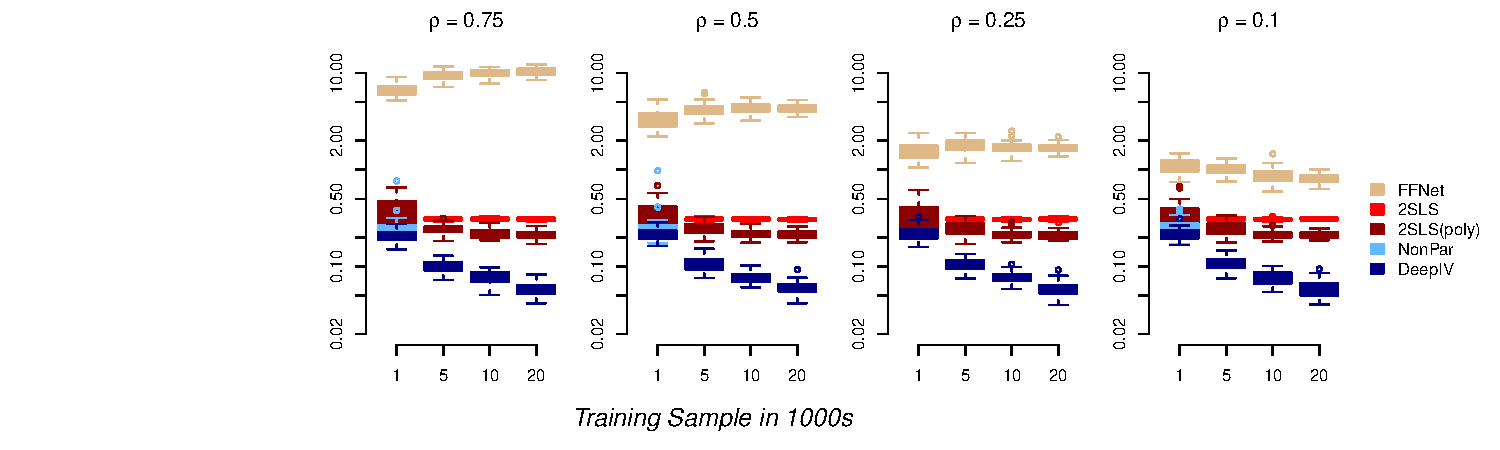
\includegraphics[width=1.1\textwidth]{figures/store}}%
        \end{figure}

    \end{frame}

    \begin{frame}{Results: Price Sensitivity with Image Features}


        \begin{minipage}[c]{0.5\textwidth}
            \begin{figure}
                \centering
                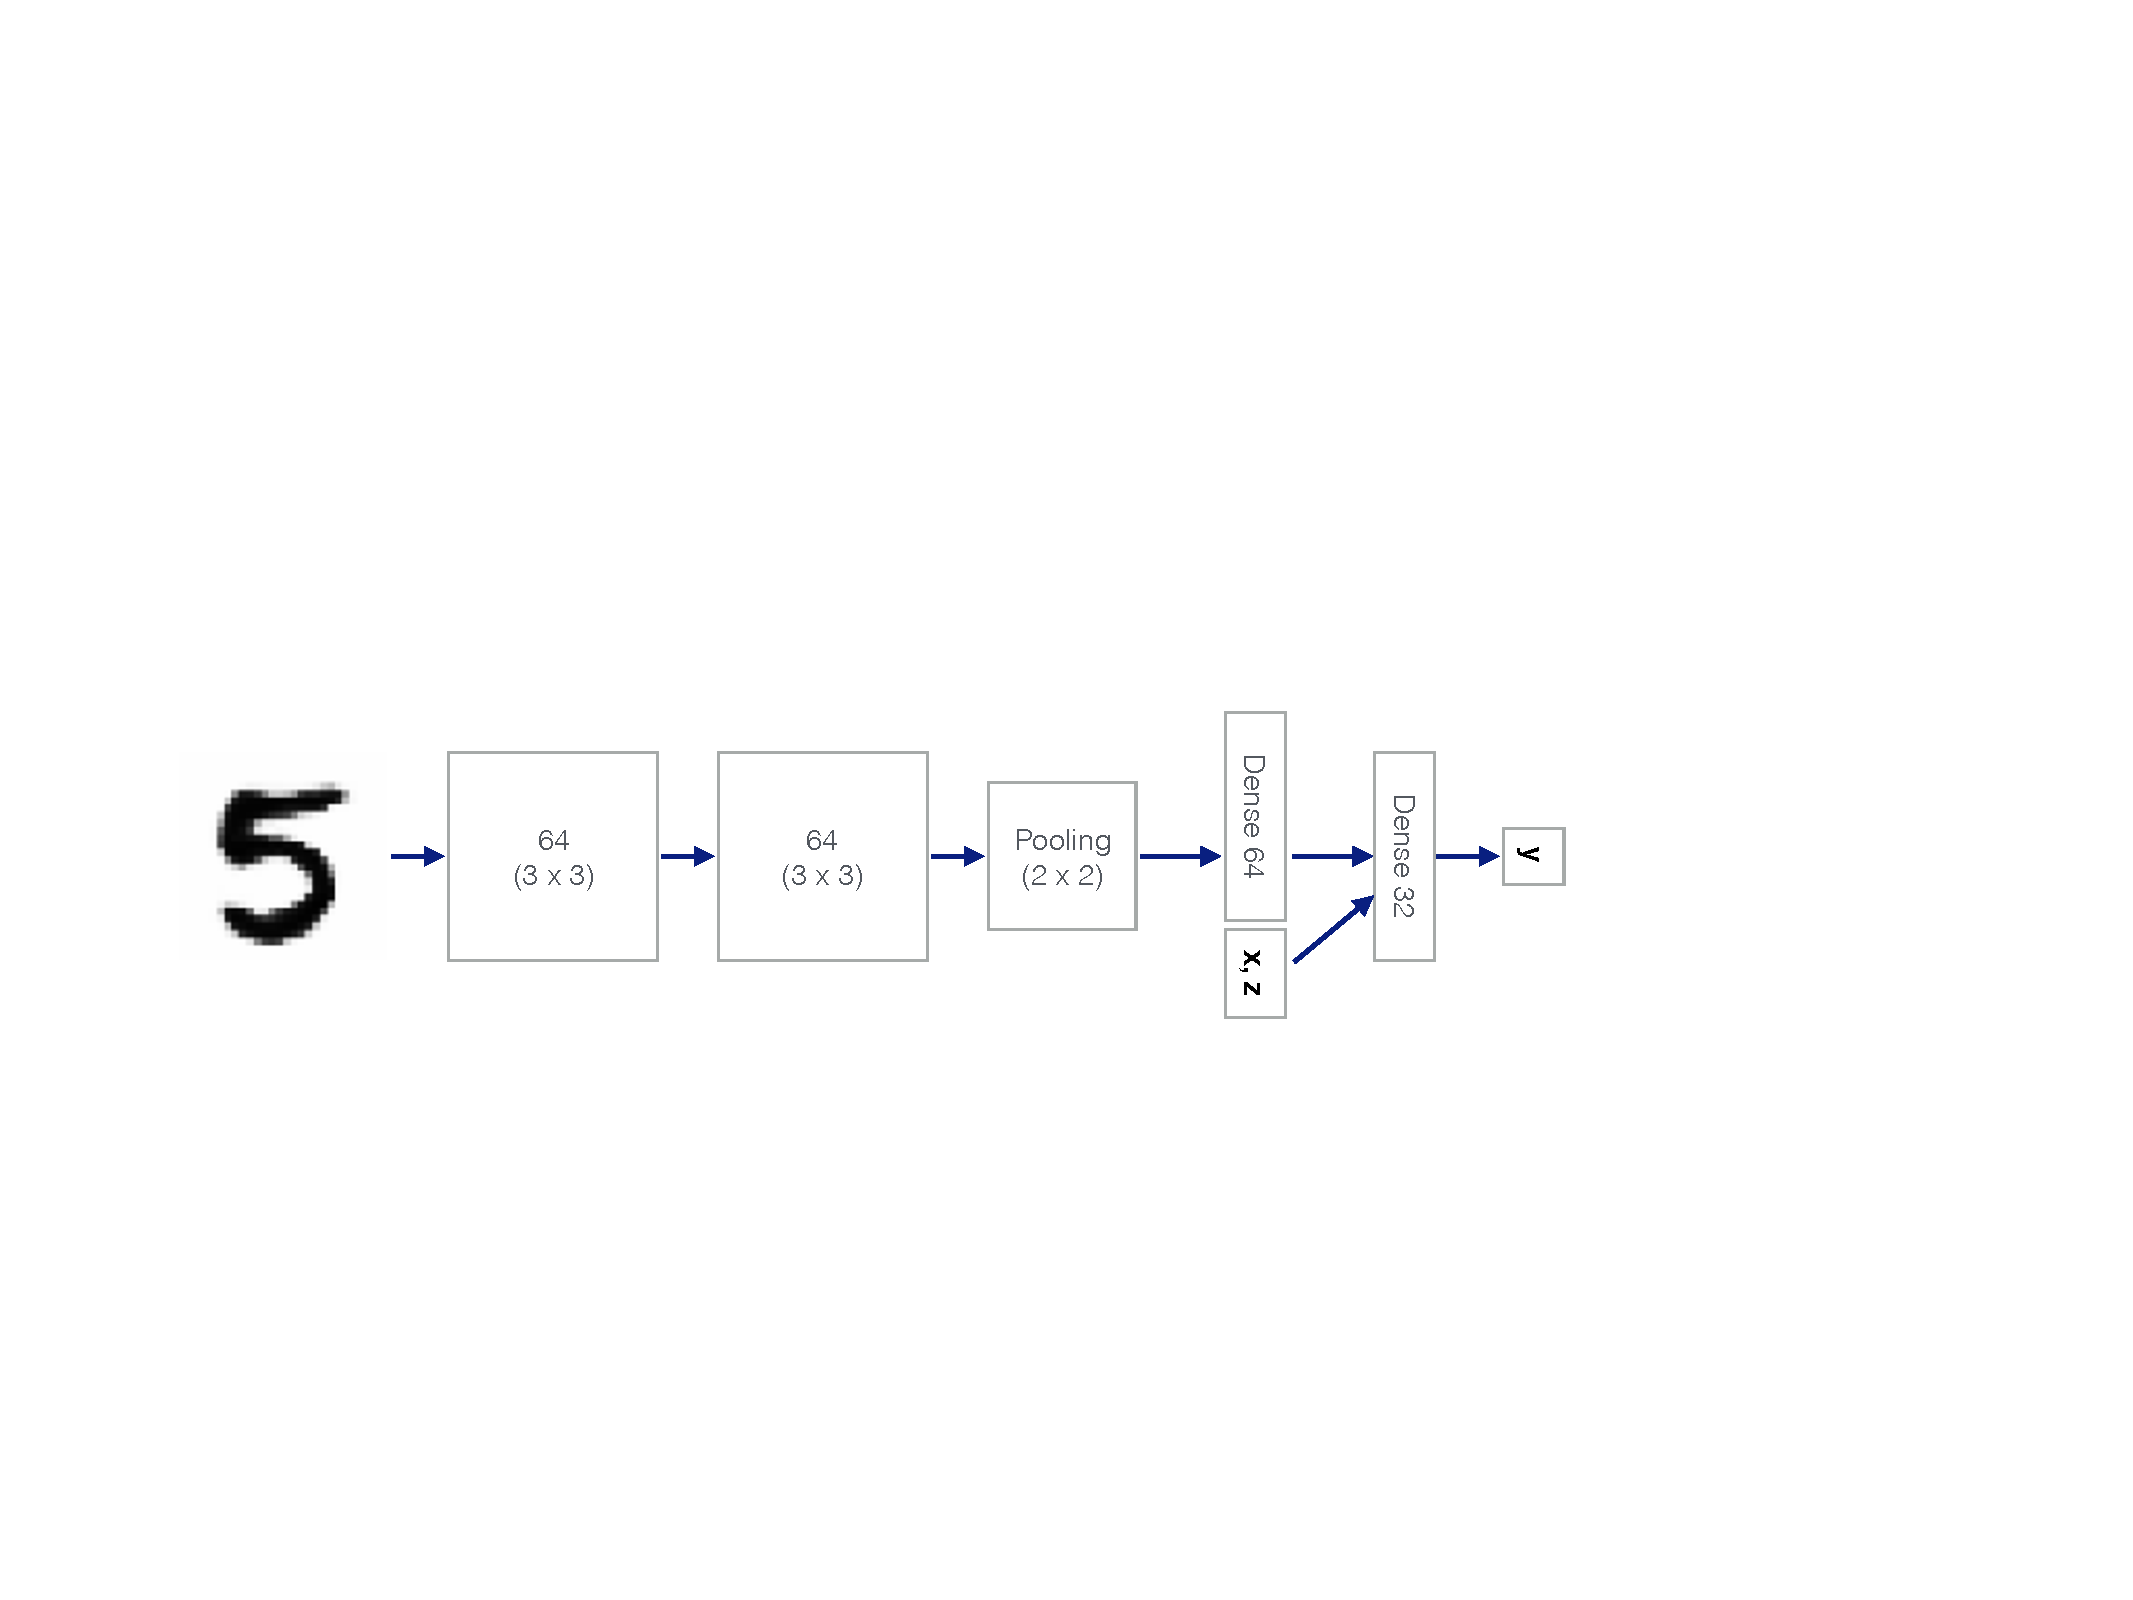
\includegraphics[width=1.5\textwidth, angle=90]{figures/convnet}
            \end{figure}

        \end{minipage}\hspace{0.1cm}
        \begin{minipage}[c]{0.45\textwidth}
            What if $S$ is an \textbf{MNIST digit?}
            \begin{figure}
                \centering
                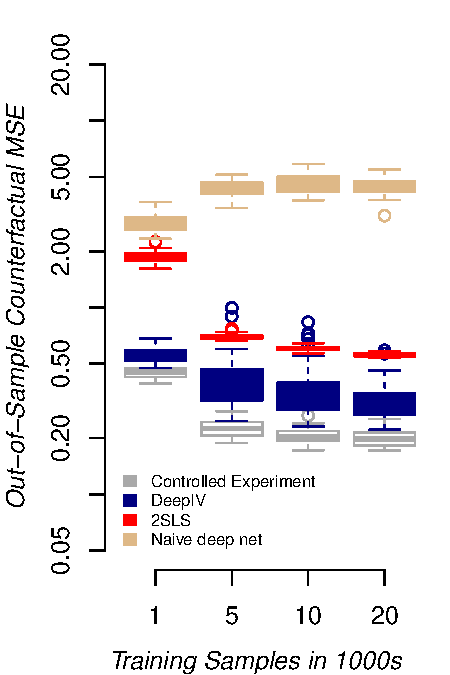
\includegraphics[width=\textwidth]{figures/image_experiment}
            \end{figure}
        \end{minipage}

    \end{frame}

    \begin{frame}{Results: Any Issues?}

        \begin{center}
            \huge Did we do something wrong?
        \end{center}

    \end{frame}

    \begin{frame}{A Forbidden Regression}
        \begin{center}
            \Large
            ``Forbidden regressions were forbidden by MIT Professor Jerry Hausman in 1975, and while they occasionally resurface in an under-supervised thesis, they are still technically off-limits.''\\
            ---\citet{angrist2008mostly}
        \end{center}
    \end{frame}

    \begin{frame}{Forbidden Regression: 2SLS vs DeepIV}
        Let \( f \) be some (non-linear) function and consider
        \begin{align*}
            h(\policy{}, \features{}) &= \mathbf{w}_0^\top \policy{} + \mathbf{w}_1^\top \features{} + \confounder{}\\
            \E[\policy{} \mid \features{}, \instrument{}] &= f\;(\features{}, \instrument{}, \confounder{}),
        \end{align*}\vspace{0.05cm}

        \textbf{Amazing Property}: 2SLS is consistent if \( h \) is linear even if \( f \) isn't!
        \begin{itemize}
            \item Prove using \textbf{orthogonality} of residual and prediction.\vspace{0.4cm}
        \end{itemize}
        \textbf{Deep IV}: bias from \( \hat p \,(\policy{} \mid \phi(\features{}, \instrument{})\,) \) propagates to \( \hat h_\theta (\policy{}, \features{})\).
        \begin{itemize}
            \item Asymptotically OK if density estimation is \textbf{realizable}.
        \end{itemize}

        \source{See \href{http://web.hku.hk/~pingyu/6005/LN/LN5_Least\%20Squares\%20Estimation-\%20Large-Sample\%20Properties.pdf}{\textcolor{blue}{\underline{this PDF}}} for a hint on how to proceed.}
    \end{frame}

    \begin{frame}{Recap}
        \large
        {\Large Today:}
        \begin{itemize}
            \item Our \textbf{goal} was counterfactual reasoning from observations.\vspace{0.2cm}
            \item Naive \textbf{supervised learning} can fail catastrophically due to confounders. \vspace{0.2cm}
            \item \textbf{Probabilistic counterfactuals} are possible with persistent confounders. \vspace{0.2cm}
            \item \textbf{Instrumental variables} allow counterfactual inference when confounders are unknown. \vspace{0.2cm}
            \item \textbf{Deep IV} uses instrumental variables with neural networks for flexible counterfactual reasoning.
        \end{itemize}
    \end{frame}

    \begin{frame}{Questions?}

        \begin{figure}
            \centering
            
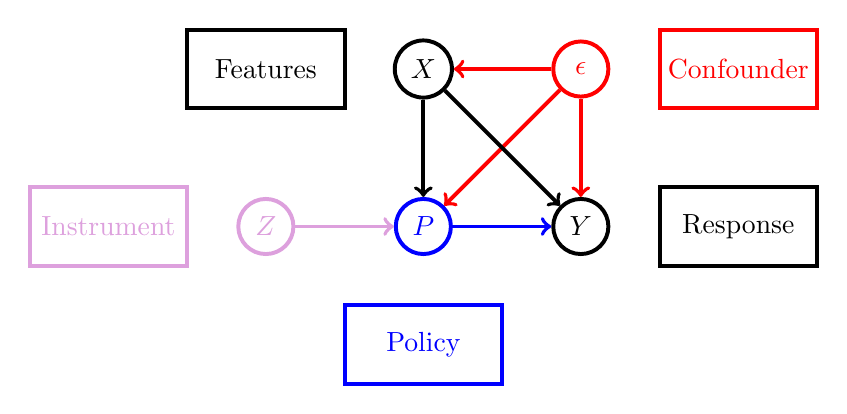
\begin{tikzpicture}
	\begin{pgfonlayer}{nodelayer}
		\node [style=Instrument] (instrument) at (-2, 0) {$Z$};
		\node [style=Endogenous] (features) at (0, 2) {$X$};
		\node [style=Endogenous] (outcomes) at (2, 0) {$Y$};
		\node [style=Policy] (policy) at (0, 0) {$P$};
		\node [style=Confounder] (confounder) at (2, 2) {$\epsilon$};
	\end{pgfonlayer}
	\begin{pgfonlayer}{edgelayer}
		\draw [->, style=arrow, draw=red] (confounder) to (policy);
		\draw [->, style=arrow, draw=red] (confounder) to (outcomes);
		\draw [->, style=arrow, draw=red] (confounder) to (features);
		\draw [->, style=arrow, draw=blue] (policy) to (outcomes);
		\draw [->, style=arrow, draw=black] (features) to (outcomes);
		\draw [->, style=arrow, draw=black] (features) to (policy);
		\draw [->, style=arrow, draw=Plum] (instrument) to (policy);

		% colored labels
		\draw [draw=red, line width = 0.5mm] (3,2.5) rectangle (5,1.5) node[pos=0.5] {\color{red}{Confounder}};
		\draw [draw=black, line width = 0.5mm] (3,0.5) rectangle (5,-0.5) node[pos=0.5] {\color{black}{Response}};
		\draw [draw=black, line width = 0.5mm] (-3,2.5) rectangle (-1,1.5) node[pos=0.5] {\color{black}{Features}};
		\draw [draw=blue, line width = 0.5mm] (-1,-1) rectangle (1,-2) node[pos=0.5] {\color{blue}{Policy}};
		\draw [draw=Plum, line width = 0.5mm] (-5,0.5) rectangle (-3,-0.5) node[pos=0.5] {\color{Plum}{Instrument}};
	\end{pgfonlayer}
\end{tikzpicture}

        \end{figure}

    \end{frame}

    % bibliography

    \begin{frame}[allowframebreaks]{References}
        \bibliographystyle{plainnat}
        \bibliography{refs}
    \end{frame}

\end{document}
